\documentclass[12pt]{article}
\usepackage{graphics}
\title{Key West Annual Mean Temperature Results}
\author{Eva Linehan}
\date{October 2018}
\begin{document}
  \maketitle
  
  \section{Objectives}
  The purpose of this exercise was to investigate if there was a correlation in mean annual temperature between successive years of the 20th century in Key West, Florida, USA.  
  
  \section{Results and Interpretation}
  The correlation coefficient between successive years was 0.326 which signifies a weak positive relationship. To investigate the significance of this correlation, the coefficient was compared to the correlation coeffients of the randomly permuted time series (n=10000). The fraction of random time series correlations greater than the successive years correlation coefficient was $6e^-4$. This suggests that the weak positive relationship identified between years is more significant than comparing the correlation between random years.
  In figure 1, the correlation coefficient of successive years was compared to the distribution of random correlation coefficients. This illustrates that the successive years correlation differs from random and is significant.
  
  \begin{figure}[h]
  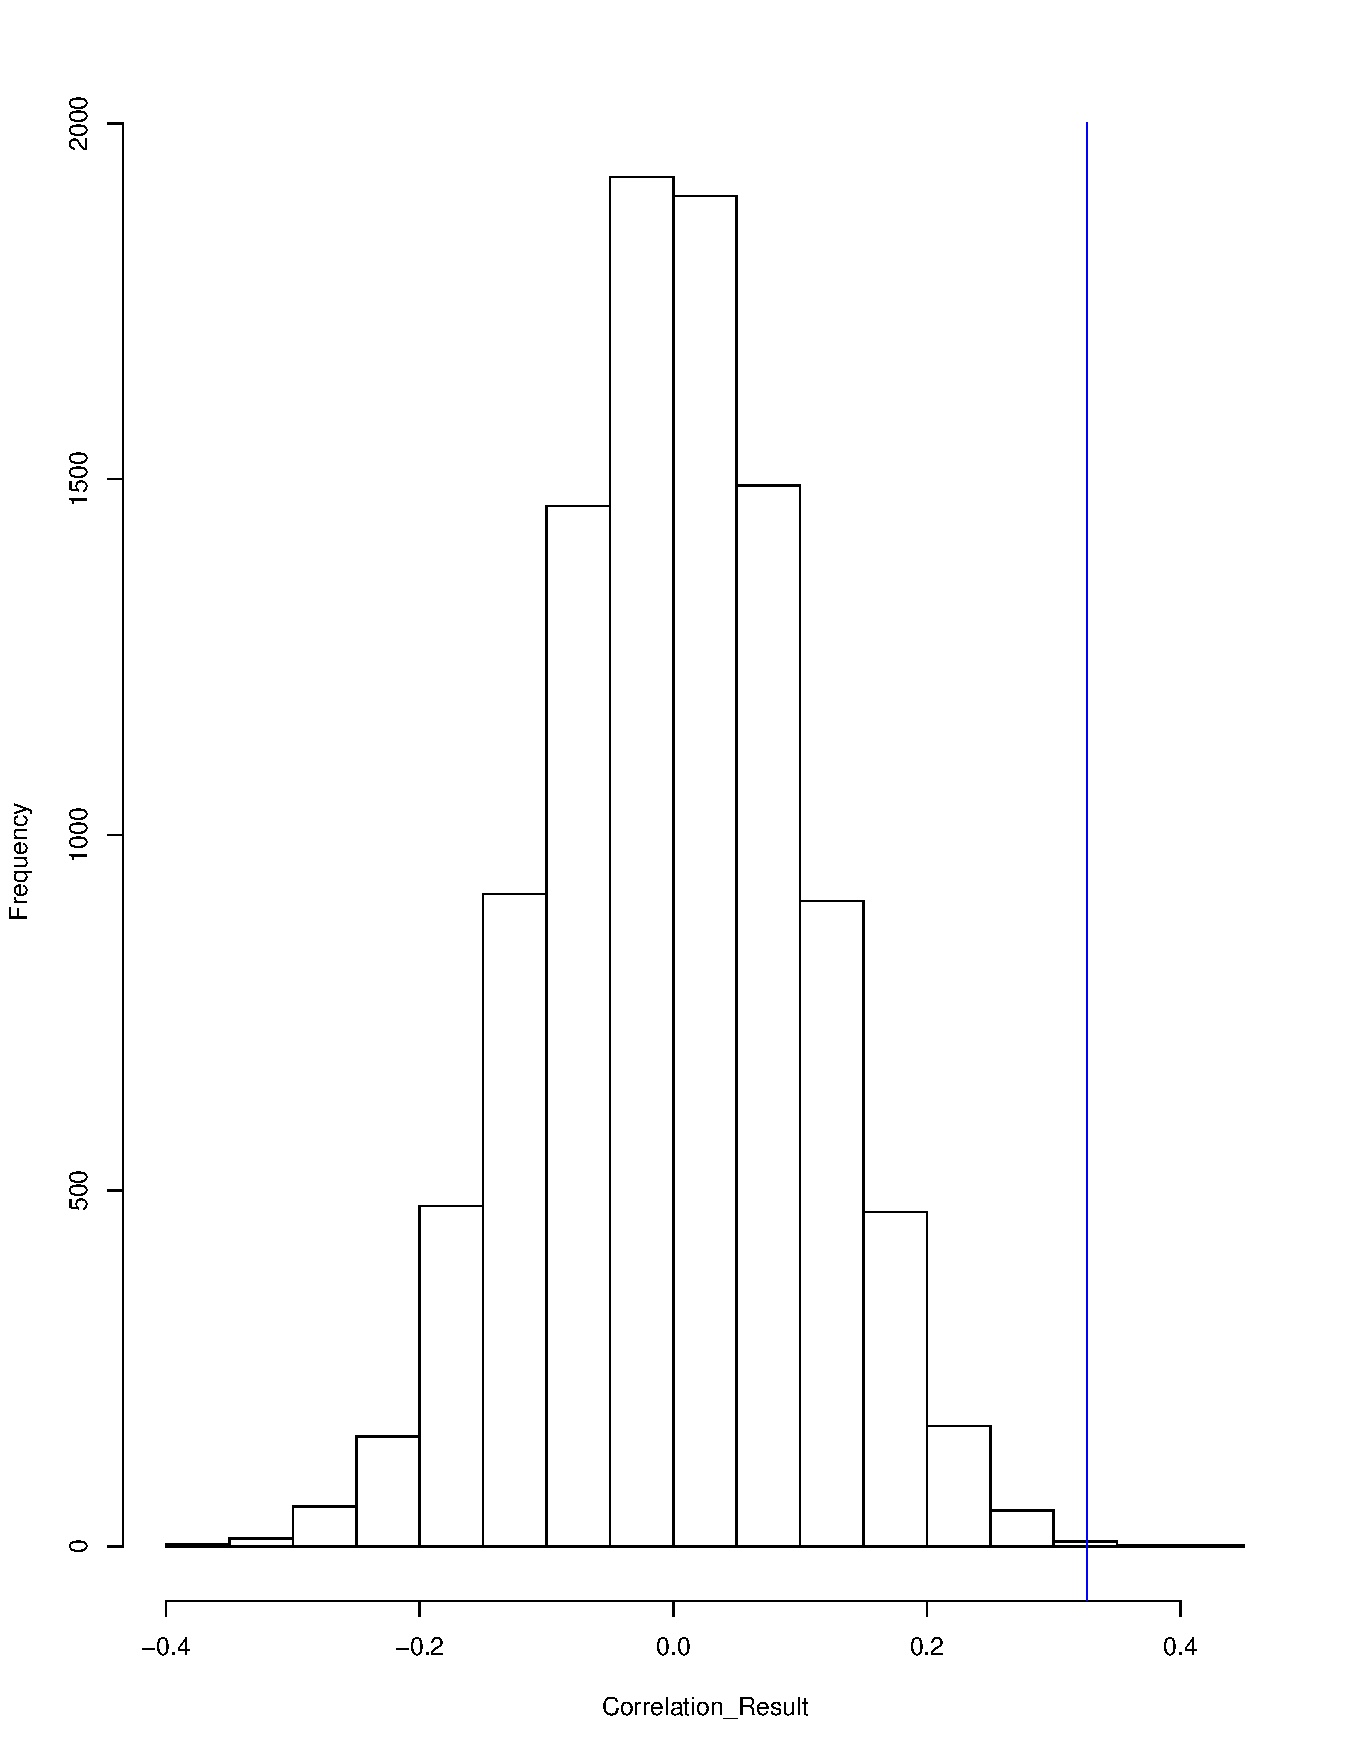
\includegraphics[width=\linewidth]{../Data/TAutoCorr_hist.pdf}
  \caption{The distribution of correlation coefficients of each randonly permuted time sequence of mean annual temperatures in Key West, Florida, USA for the 20th century. The blue line signifies the position of the correlation coefficient of successive years in the random z-distribution.}
  \end{figure}[h]
\end{document}

	content...
